\batchmode
\makeatletter
\def\input@path{{/Users/altuna/Dropbox/PAPERS/R-devel/compgenr/chapters//}}
\makeatother
\documentclass[english,nohyper]{tufte-book}\usepackage[]{graphicx}\usepackage[]{color}
%% maxwidth is the original width if it is less than linewidth
%% otherwise use linewidth (to make sure the graphics do not exceed the margin)
\makeatletter
\def\maxwidth{ %
  \ifdim\Gin@nat@width>\linewidth
    \linewidth
  \else
    \Gin@nat@width
  \fi
}
\makeatother

\definecolor{fgcolor}{rgb}{0.345, 0.345, 0.345}
\newcommand{\hlnum}[1]{\textcolor[rgb]{0.686,0.059,0.569}{#1}}%
\newcommand{\hlstr}[1]{\textcolor[rgb]{0.192,0.494,0.8}{#1}}%
\newcommand{\hlcom}[1]{\textcolor[rgb]{0.678,0.584,0.686}{\textit{#1}}}%
\newcommand{\hlopt}[1]{\textcolor[rgb]{0,0,0}{#1}}%
\newcommand{\hlstd}[1]{\textcolor[rgb]{0.345,0.345,0.345}{#1}}%
\newcommand{\hlkwa}[1]{\textcolor[rgb]{0.161,0.373,0.58}{\textbf{#1}}}%
\newcommand{\hlkwb}[1]{\textcolor[rgb]{0.69,0.353,0.396}{#1}}%
\newcommand{\hlkwc}[1]{\textcolor[rgb]{0.333,0.667,0.333}{#1}}%
\newcommand{\hlkwd}[1]{\textcolor[rgb]{0.737,0.353,0.396}{\textbf{#1}}}%

\usepackage{framed}
\makeatletter
\newenvironment{kframe}{%
 \def\at@end@of@kframe{}%
 \ifinner\ifhmode%
  \def\at@end@of@kframe{\end{minipage}}%
  \begin{minipage}{\columnwidth}%
 \fi\fi%
 \def\FrameCommand##1{\hskip\@totalleftmargin \hskip-\fboxsep
 \colorbox{shadecolor}{##1}\hskip-\fboxsep
     % There is no \\@totalrightmargin, so:
     \hskip-\linewidth \hskip-\@totalleftmargin \hskip\columnwidth}%
 \MakeFramed {\advance\hsize-\width
   \@totalleftmargin\z@ \linewidth\hsize
   \@setminipage}}%
 {\par\unskip\endMakeFramed%
 \at@end@of@kframe}
\makeatother

\definecolor{shadecolor}{rgb}{.97, .97, .97}
\definecolor{messagecolor}{rgb}{0, 0, 0}
\definecolor{warningcolor}{rgb}{1, 0, 1}
\definecolor{errorcolor}{rgb}{1, 0, 0}
\newenvironment{knitrout}{}{} % an empty environment to be redefined in TeX

\usepackage{alltt}
\usepackage[T1]{fontenc}
\usepackage[latin9]{inputenc}
\synctex=-1
\usepackage{babel}
\usepackage{url}
\usepackage{graphicx}
\PassOptionsToPackage{normalem}{ulem}
\usepackage{ulem}
\usepackage[unicode=true,pdfusetitle,
 bookmarks=true,bookmarksnumbered=false,bookmarksopen=false,
 breaklinks=false,pdfborder={0 0 1},backref=false,colorlinks=false]
 {hyperref}
\IfFileExists{upquote.sty}{\usepackage{upquote}}{}
\begin{document}






\chapter{Quick introduction to R}

R is a free statistical programming language that is popular among
researchers and data miners to build software and analyze data%
\footnote{if you want to know more about details about R and its history here
is a good place to start \url{http://en.wikipedia.org/wiki/R_(programming_language)}%
}. In next sections, we will first get you started with the setup of
environment for using R and then introduce some basic R operations
and data structures that will be good to know if you do not have prior
experience with R. If you need more in depth R introduction you will
want to check out some beginner level books and online tutorials.
This website has a bunch of resources listed: \url{http://www.introductoryr.co.uk/R_Resources_for_Beginners.html}


\section{The setup}

Download and install R \url{http://cran.r-project.org/} and RStudio
\url{http://www.rstudio.com/} if you do not have them already. Rstudio
is optional but it is a great tool if you are just starting to learn
R. You will need specific data sets to run the codes in this document.
Download the data.zip{[}URL to come{]} and extract it to your directory
of choice. The folder name should be ``data'' and your R working
directory should be level above the data folder. That means in your
R console, when you type ``\emph{dir(``data'')}'' you should be
able to see the contents of the data folder. You can change your working
directory by \emph{setwd()} command and get your current working directory
with \emph{getwd()} command in R%
\footnote{\uline{TIP:} dir() gives you files in your current working directory.
getwd() gets current directory. You may need these at some point. %
}. In RStudio, you can click on the top menu and change the location
of your working directory via user interface.


\subsection{Installing packages}

R packages are add-ons to base R that help you achieve additional
tasks that are not directly supported by base R. It is by the action
of these extra functionality that R excels as a tool for computational
genomics. Bioconductor project (\url{http://bioconductor.org/}) is
a dedicated package repository for computational biology related packages.
However main package repository of R, called CRAN, has also computational
biology related packages. In addition, R-Forge(\url{http://r-forge.r-project.org/}),
GitHub(\url{https://github.com/}), and googlecode(\url{http://code.google.com})
are other locations where R packages might be hosted.

You can install CRAN packages using install.packages(). (\# is the
comment character in R)

\begin{knitrout}
\definecolor{shadecolor}{rgb}{0.969, 0.969, 0.969}\color{fgcolor}\begin{kframe}
\begin{alltt}
\hlcom{# install package named 'randomForests' from CRAN}
\hlkwd{install.packages}\hlstd{(}\hlstr{"randomForests"}\hlstd{)}
\end{alltt}
\end{kframe}
\end{knitrout}


You can install packages from bioconductor with their specific installer
script.

\begin{knitrout}
\definecolor{shadecolor}{rgb}{0.969, 0.969, 0.969}\color{fgcolor}\begin{kframe}
\begin{alltt}
\hlcom{# get the installer package}
\hlkwd{source}\hlstd{(}\hlstr{"http://bioconductor.org/biocLite.R"}\hlstd{)}
\hlcom{# install bioconductor package 'rtracklayer'}
\hlkwd{biocLite}\hlstd{(}\hlstr{"rtracklayer"}\hlstd{)}
\end{alltt}
\end{kframe}
\end{knitrout}


Installing packages from GitHub via install\_github function from
devtools package.

\begin{knitrout}
\definecolor{shadecolor}{rgb}{0.969, 0.969, 0.969}\color{fgcolor}\begin{kframe}
\begin{alltt}
\hlkwd{library}\hlstd{(devtools)}
\hlkwd{install_github}\hlstd{(}\hlstr{"roxygen"}\hlstd{)}
\end{alltt}
\end{kframe}
\end{knitrout}


You can install packages from the source files, that usually have
.tar.gz suffix.

\begin{knitrout}
\definecolor{shadecolor}{rgb}{0.969, 0.969, 0.969}\color{fgcolor}\begin{kframe}
\begin{alltt}
\hlcom{# download the source file}
\hlkwd{download.file}\hlstd{(}\hlstr{"http://goo.gl/3pvHYI"}\hlstd{,}
               \hlkwc{destfile}\hlstd{=}\hlstr{"methylKit_0.5.7.tar.gz"}\hlstd{)}
\hlcom{# install the package from the source file}
\hlkwd{install.packages}\hlstd{(}\hlstr{"methylKit_0.5.7.tar.gz"}\hlstd{,}
                 \hlkwc{repos}\hlstd{=}\hlkwa{NULL}\hlstd{,}\hlkwc{type}\hlstd{=}\hlstr{"source"}\hlstd{)}
\hlcom{# delete the source file}
\hlkwd{unlink}\hlstd{(}\hlstr{"methylKit_0.5.7.tar.gz"}\hlstd{)}
\end{alltt}
\end{kframe}
\end{knitrout}


You can also update installed packages from CRAN and Bioconductor.

\begin{knitrout}
\definecolor{shadecolor}{rgb}{0.969, 0.969, 0.969}\color{fgcolor}\begin{kframe}
\begin{alltt}
\hlcom{# updating CRAN packages}
\hlkwd{update.packages}\hlstd{()}
\hlcom{# updating bioconductor packages}
\hlkwd{source}\hlstd{(}\hlstr{"http://bioconductor.org/biocLite.R"}\hlstd{)}
\hlkwd{biocLite}\hlstd{(}\hlstr{"BiocUpgrade"}\hlstd{)}
\end{alltt}
\end{kframe}
\end{knitrout}



\subsection{installing packages in custom locations}

If you will be using R on servers or computing clusters rather than
your personal computer it is unlikey that you will have administrator
access to install packages. In that case, you can install packges
in custom locations by telling R where to look for additional packages.
This is done by setting up an \emph{.Renviron} file in your home directory
and add the following line:

\begin{verbatim}
R_LIBS=~/Rlibs
\end{verbatim}

This tells R that ``Rlibs'' directory at your home directory will
be the first choice of locations to look for packages and install
packages (The directory name and location is up to you above is just
an example). You should go and create that directory now. After that,
start a fresh R session and start installing packages. From now on,
packages will be installed to your local directory where you have
read-write access.


\subsection{Getting help on R functions and packages}

You can get help on functions by help() and help.search() functions.
You can list the functions in a package with ls() function

\begin{knitrout}
\definecolor{shadecolor}{rgb}{0.969, 0.969, 0.969}\color{fgcolor}\begin{kframe}
\begin{alltt}
\hlkwd{libray}\hlstd{(MASS)}
\hlkwd{ls}\hlstd{(}\hlstr{"package:MASS"}\hlstd{)}  \hlcom{# functions in the package}
\hlkwd{ls}\hlstd{()}  \hlcom{# objects in your R enviroment}
\hlcom{# get help on hist() function}
\hlkwd{`?`}\hlstd{(hist)}
\hlkwd{help}\hlstd{(}\hlstr{"hist"}\hlstd{)}
\hlcom{# search the word 'hist' in help pages}
\hlkwd{help.search}\hlstd{(}\hlstr{"hist"}\hlstd{)}
\hlkwd{`?`}\hlstd{(}\hlkwd{`?`}\hlstd{(hist))}
\end{alltt}
\end{kframe}
\end{knitrout}


In addition, check \uline{package vignettes} for help and practical
understanding of the functions. All Bionconductor packages have vignettes
that walk you thorugh example analysis. \uline{Google search} will
always be helpful as well, there are many blogs and web pages that
have posts about R.


\section{Computations in R}

R can be used as an ordinary calculator. Here are a few examples:

\begin{knitrout}
\definecolor{shadecolor}{rgb}{0.969, 0.969, 0.969}\color{fgcolor}\begin{kframe}
\begin{alltt}
\hlnum{2} \hlopt{+} \hlnum{3} \hlopt{*} \hlnum{5}  \hlcom{# Note the order of operations. }
\end{alltt}
\begin{verbatim}
## [1] 17
\end{verbatim}
\begin{alltt}
\hlkwd{log}\hlstd{(}\hlnum{10}\hlstd{)}  \hlcom{# Natural logarithm with base e}
\end{alltt}
\begin{verbatim}
## [1] 2.303
\end{verbatim}
\begin{alltt}
\hlnum{5}\hlopt{^}\hlnum{2}  \hlcom{# 5 raised to the second power }
\end{alltt}
\begin{verbatim}
## [1] 25
\end{verbatim}
\begin{alltt}
\hlnum{3}\hlopt{/}\hlnum{2}  \hlcom{# Division }
\end{alltt}
\begin{verbatim}
## [1] 1.5
\end{verbatim}
\begin{alltt}
\hlkwd{sqrt}\hlstd{(}\hlnum{16}\hlstd{)}  \hlcom{# Square root }
\end{alltt}
\begin{verbatim}
## [1] 4
\end{verbatim}
\begin{alltt}
\hlkwd{abs}\hlstd{(}\hlnum{3} \hlopt{-} \hlnum{7}\hlstd{)}  \hlcom{# Absolute value of 3-7 }
\end{alltt}
\begin{verbatim}
## [1] 4
\end{verbatim}
\begin{alltt}
\hlstd{pi}  \hlcom{# The number }
\end{alltt}
\begin{verbatim}
## [1] 3.142
\end{verbatim}
\begin{alltt}
\hlkwd{exp}\hlstd{(}\hlnum{2}\hlstd{)}  \hlcom{# exponential function }
\end{alltt}
\begin{verbatim}
## [1] 7.389
\end{verbatim}
\begin{alltt}
# This is a comment line
\end{alltt}
\end{kframe}
\end{knitrout}





\section{Vectors}

Vectors is one the core R data structures. R handles vectors easily
and intuitively. You can create vectors with \emph{c()} function,
however that is not the only way. The operations on vectors will propagate
to all the elements of the vectors.

\begin{knitrout}
\definecolor{shadecolor}{rgb}{0.969, 0.969, 0.969}\color{fgcolor}\begin{kframe}
\begin{alltt}
\hlstd{x} \hlkwb{<-} \hlkwd{c}\hlstd{(}\hlnum{1}\hlstd{,} \hlnum{3}\hlstd{,} \hlnum{2}\hlstd{,} \hlnum{10}\hlstd{,} \hlnum{5}\hlstd{)}  \hlcom{#create a vector x with 5 components }
\hlstd{x}
\end{alltt}
\begin{verbatim}
## [1]  1  3  2 10  5
\end{verbatim}
\begin{alltt}
\hlstd{y} \hlkwb{<-} \hlnum{1}\hlopt{:}\hlnum{5}  \hlcom{#create a vector of consecutive integers y }
\hlstd{y} \hlopt{+} \hlnum{2}  \hlcom{#scalar addition }
\end{alltt}
\begin{verbatim}
## [1] 3 4 5 6 7
\end{verbatim}
\begin{alltt}
\hlnum{2} \hlopt{*} \hlstd{y}  \hlcom{#scalar multiplication}
\end{alltt}
\begin{verbatim}
## [1]  2  4  6  8 10
\end{verbatim}
\begin{alltt}
\hlstd{y}\hlopt{^}\hlnum{2}  \hlcom{#raise each component to the second power}
\end{alltt}
\begin{verbatim}
## [1]  1  4  9 16 25
\end{verbatim}
\begin{alltt}
\hlnum{2}\hlopt{^}\hlstd{y}  \hlcom{#raise 2 to the first through fifth power }
\end{alltt}
\begin{verbatim}
## [1]  2  4  8 16 32
\end{verbatim}
\begin{alltt}
\hlstd{y}  \hlcom{#y itself has not been unchanged }
\end{alltt}
\begin{verbatim}
## [1] 1 2 3 4 5
\end{verbatim}
\begin{alltt}
\hlstd{y} \hlkwb{<-} \hlstd{y} \hlopt{*} \hlnum{2}
\hlstd{y}  \hlcom{#it is now changed}
\end{alltt}
\begin{verbatim}
## [1]  2  4  6  8 10
\end{verbatim}
\begin{alltt}
\hlstd{r1} \hlkwb{<-} \hlkwd{rep}\hlstd{(}\hlnum{1}\hlstd{,} \hlnum{3}\hlstd{)}  \hlcom{# create a vector of 1s, length 3 }
\hlkwd{length}\hlstd{(r1)}  \hlcom{#length of the vector}
\end{alltt}
\begin{verbatim}
## [1] 3
\end{verbatim}
\begin{alltt}
\hlkwd{class}\hlstd{(r1)}  \hlcom{# class of the vector}
\end{alltt}
\begin{verbatim}
## [1] "numeric"
\end{verbatim}
\begin{alltt}
\hlstd{a} \hlkwb{<-} \hlnum{1}  \hlcom{# this is actually a vector length one}
\end{alltt}
\end{kframe}
\end{knitrout}



\subsection{Data types in R}

There are four comon data types in R, they are numeric, logical and
character and integer. All these data types can be used to create
vectors natively.

\begin{knitrout}
\definecolor{shadecolor}{rgb}{0.969, 0.969, 0.969}\color{fgcolor}\begin{kframe}
\begin{alltt}
\hlcom{# create a numeric vector x with 5 components}
\hlstd{x} \hlkwb{<-} \hlkwd{c}\hlstd{(}\hlnum{1}\hlstd{,} \hlnum{3}\hlstd{,} \hlnum{2}\hlstd{,} \hlnum{10}\hlstd{,} \hlnum{5}\hlstd{)}
\hlstd{x}
\end{alltt}
\begin{verbatim}
## [1]  1  3  2 10  5
\end{verbatim}
\begin{alltt}
\hlcom{# create a logical vector x}
\hlstd{x} \hlkwb{<-} \hlkwd{c}\hlstd{(}\hlnum{TRUE}\hlstd{,} \hlnum{FALSE}\hlstd{,} \hlnum{TRUE}\hlstd{)}
\hlstd{x}
\end{alltt}
\begin{verbatim}
## [1]  TRUE FALSE  TRUE
\end{verbatim}
\begin{alltt}
\hlcom{# create a character vector}
\hlstd{x} \hlkwb{<-} \hlkwd{c}\hlstd{(}\hlstr{"sds"}\hlstd{,} \hlstr{"sd"}\hlstd{,} \hlstr{"as"}\hlstd{)}
\hlstd{x}
\end{alltt}
\begin{verbatim}
## [1] "sds" "sd"  "as"
\end{verbatim}
\begin{alltt}
\hlkwd{class}\hlstd{(x)}
\end{alltt}
\begin{verbatim}
## [1] "character"
\end{verbatim}
\begin{alltt}
\hlcom{# create an integer vector}
\hlstd{x} \hlkwb{<-} \hlkwd{c}\hlstd{(}\hlnum{1L}\hlstd{,} \hlnum{2L}\hlstd{,} \hlnum{3L}\hlstd{)}
\hlstd{x}
\end{alltt}
\begin{verbatim}
## [1] 1 2 3
\end{verbatim}
\begin{alltt}
\hlkwd{class}\hlstd{(x)}
\end{alltt}
\begin{verbatim}
## [1] "integer"
\end{verbatim}
\end{kframe}
\end{knitrout}



\section{Matrices}

A matrix refers to a numeric array of rows and columns. You can think
of it as a stacked version of vectors where each row or column is
a vector. One of the easiest ways to create a matrix is to combine
vectors of equal length using \emph{cbind()}, meaning 'column bind'

\begin{knitrout}
\definecolor{shadecolor}{rgb}{0.969, 0.969, 0.969}\color{fgcolor}\begin{kframe}
\begin{alltt}
\hlstd{x} \hlkwb{<-} \hlkwd{c}\hlstd{(}\hlnum{1}\hlstd{,} \hlnum{2}\hlstd{,} \hlnum{3}\hlstd{,} \hlnum{4}\hlstd{)}
\hlstd{y} \hlkwb{<-} \hlkwd{c}\hlstd{(}\hlnum{4}\hlstd{,} \hlnum{5}\hlstd{,} \hlnum{6}\hlstd{,} \hlnum{7}\hlstd{)}
\hlstd{m1} \hlkwb{<-} \hlkwd{cbind}\hlstd{(x, y)}
\hlstd{m1}
\end{alltt}
\begin{verbatim}
##      x y
## [1,] 1 4
## [2,] 2 5
## [3,] 3 6
## [4,] 4 7
\end{verbatim}
\begin{alltt}
\hlkwd{t}\hlstd{(m1)}  \hlcom{# transpose of m1}
\end{alltt}
\begin{verbatim}
##   [,1] [,2] [,3] [,4]
## x    1    2    3    4
## y    4    5    6    7
\end{verbatim}
\begin{alltt}
\hlkwd{dim}\hlstd{(m1)}  \hlcom{# 2 by 5 matrix }
\end{alltt}
\begin{verbatim}
## [1] 4 2
\end{verbatim}
\end{kframe}
\end{knitrout}


You can also directly list the elements and specify the matrix:

\begin{knitrout}
\definecolor{shadecolor}{rgb}{0.969, 0.969, 0.969}\color{fgcolor}\begin{kframe}
\begin{alltt}
\hlstd{m2} \hlkwb{<-} \hlkwd{matrix}\hlstd{(}\hlkwd{c}\hlstd{(}\hlnum{1}\hlstd{,} \hlnum{3}\hlstd{,} \hlnum{2}\hlstd{,} \hlnum{5}\hlstd{,} \hlopt{-}\hlnum{1}\hlstd{,} \hlnum{2}\hlstd{,} \hlnum{2}\hlstd{,} \hlnum{3}\hlstd{,} \hlnum{9}\hlstd{),} \hlkwc{nrow} \hlstd{=} \hlnum{3}\hlstd{)}
\hlstd{m2}
\end{alltt}
\begin{verbatim}
##      [,1] [,2] [,3]
## [1,]    1    5    2
## [2,]    3   -1    3
## [3,]    2    2    9
\end{verbatim}
\end{kframe}
\end{knitrout}



\section{Data Frames}

A data frame is more general than a matrix, in that different columns
can have different modes (numeric, character, factor, etc.). A data
frame can be constructed by \emph{data.frame()} function. For example,
we illustrate how to construct a data frame from genomic intervals
or coordinates.

\begin{knitrout}
\definecolor{shadecolor}{rgb}{0.969, 0.969, 0.969}\color{fgcolor}\begin{kframe}
\begin{alltt}
\hlstd{chr} \hlkwb{<-} \hlkwd{c}\hlstd{(}\hlstr{"chr1"}\hlstd{,} \hlstr{"chr1"}\hlstd{,} \hlstr{"chr2"}\hlstd{,} \hlstr{"chr2"}\hlstd{)}
\hlstd{strand} \hlkwb{<-} \hlkwd{c}\hlstd{(}\hlstr{"-"}\hlstd{,} \hlstr{"-"}\hlstd{,} \hlstr{"+"}\hlstd{,} \hlstr{"+"}\hlstd{)}
\hlstd{start} \hlkwb{<-} \hlkwd{c}\hlstd{(}\hlnum{200}\hlstd{,} \hlnum{4000}\hlstd{,} \hlnum{100}\hlstd{,} \hlnum{400}\hlstd{)}
\hlstd{end} \hlkwb{<-} \hlkwd{c}\hlstd{(}\hlnum{250}\hlstd{,} \hlnum{410}\hlstd{,} \hlnum{200}\hlstd{,} \hlnum{450}\hlstd{)}
\hlstd{mydata} \hlkwb{<-} \hlkwd{data.frame}\hlstd{(chr, start, end, strand)}
\hlcom{# change column names}
\hlkwd{names}\hlstd{(mydata)} \hlkwb{<-} \hlkwd{c}\hlstd{(}\hlstr{"chr"}\hlstd{,} \hlstr{"start"}\hlstd{,} \hlstr{"end"}\hlstd{,} \hlstr{"strand"}\hlstd{)}
\hlstd{mydata}  \hlcom{# OR this will work too }
\end{alltt}
\begin{verbatim}
##    chr start end strand
## 1 chr1   200 250      -
## 2 chr1  4000 410      -
## 3 chr2   100 200      +
## 4 chr2   400 450      +
\end{verbatim}
\begin{alltt}
\hlstd{mydata} \hlkwb{<-} \hlkwd{data.frame}\hlstd{(}\hlkwc{chr} \hlstd{= chr,} \hlkwc{start} \hlstd{= start,} \hlkwc{end} \hlstd{= end,}
    \hlkwc{strand} \hlstd{= strand)}
\hlstd{mydata}
\end{alltt}
\begin{verbatim}
##    chr start end strand
## 1 chr1   200 250      -
## 2 chr1  4000 410      -
## 3 chr2   100 200      +
## 4 chr2   400 450      +
\end{verbatim}
\end{kframe}
\end{knitrout}


There are a variety of ways to extract the elements of a data frame.
You can extract certain columns using column numbers or names, or
you can extract certain rows by using row numbers. You can also extract
data using logical arguments, such as extracting all rows that has
a value in a column larger than your threshold.

\begin{knitrout}
\definecolor{shadecolor}{rgb}{0.969, 0.969, 0.969}\color{fgcolor}\begin{kframe}
\begin{alltt}
\hlstd{mydata[,} \hlnum{2}\hlopt{:}\hlnum{4}\hlstd{]}  \hlcom{# columns 2,3,4 of data frame }
\end{alltt}
\begin{verbatim}
##   start end strand
## 1   200 250      -
## 2  4000 410      -
## 3   100 200      +
## 4   400 450      +
\end{verbatim}
\begin{alltt}
\hlstd{mydata[,} \hlkwd{c}\hlstd{(}\hlstr{"chr"}\hlstd{,} \hlstr{"start"}\hlstd{)]}  \hlcom{# columns chr and start from data frame }
\end{alltt}
\begin{verbatim}
##    chr start
## 1 chr1   200
## 2 chr1  4000
## 3 chr2   100
## 4 chr2   400
\end{verbatim}
\begin{alltt}
\hlstd{mydata}\hlopt{$}\hlstd{start}  \hlcom{# variable start in the data frame }
\end{alltt}
\begin{verbatim}
## [1]  200 4000  100  400
\end{verbatim}
\begin{alltt}
\hlstd{mydata[}\hlkwd{c}\hlstd{(}\hlnum{1}\hlstd{,} \hlnum{3}\hlstd{), ]}  \hlcom{# get 1st and 3rd rows }
\end{alltt}
\begin{verbatim}
##    chr start end strand
## 1 chr1   200 250      -
## 3 chr2   100 200      +
\end{verbatim}
\begin{alltt}
\hlstd{mydata[mydata}\hlopt{$}\hlstd{start} \hlopt{>} \hlnum{400}\hlstd{, ]}  \hlcom{# get all rows where start>400}
\end{alltt}
\begin{verbatim}
##    chr start end strand
## 2 chr1  4000 410      -
\end{verbatim}
\end{kframe}
\end{knitrout}



\section{Lists}

An ordered collection of objects (components). A list allows you to
gather a variety of (possibly unrelated) objects under one name. 

\begin{knitrout}
\definecolor{shadecolor}{rgb}{0.969, 0.969, 0.969}\color{fgcolor}\begin{kframe}
\begin{alltt}
\hlcom{# example of a list with 4 components }
\hlcom{# a string, a numeric vector, a matrix, and a scalar }
\hlstd{w} \hlkwb{<-} \hlkwd{list}\hlstd{(}\hlkwc{name}\hlstd{=}\hlstr{"Fred"}\hlstd{,}
       \hlkwc{mynumbers}\hlstd{=}\hlkwd{c}\hlstd{(}\hlnum{1}\hlstd{,}\hlnum{2}\hlstd{,}\hlnum{3}\hlstd{),}
       \hlkwc{mymatrix}\hlstd{=}\hlkwd{matrix}\hlstd{(}\hlnum{1}\hlopt{:}\hlnum{4}\hlstd{,}\hlkwc{ncol}\hlstd{=}\hlnum{2}\hlstd{),}
       \hlkwc{age}\hlstd{=}\hlnum{5.3}\hlstd{)}
\hlstd{w}
\end{alltt}
\begin{verbatim}
## $name
## [1] "Fred"
## 
## $mynumbers
## [1] 1 2 3
## 
## $mymatrix
##      [,1] [,2]
## [1,]    1    3
## [2,]    2    4
## 
## $age
## [1] 5.3
\end{verbatim}
\end{kframe}
\end{knitrout}


You can extract elements of a list using the {[}{[}{]}{]} convention
using either its position in the list or its name.

\begin{knitrout}
\definecolor{shadecolor}{rgb}{0.969, 0.969, 0.969}\color{fgcolor}\begin{kframe}
\begin{alltt}
\hlstd{w[[}\hlnum{3}\hlstd{]]}  \hlcom{# 3rd component of the list }
\end{alltt}
\begin{verbatim}
##      [,1] [,2]
## [1,]    1    3
## [2,]    2    4
\end{verbatim}
\begin{alltt}
\hlstd{w[[}\hlstr{"mynumbers"}\hlstd{]]}  \hlcom{# component named mynumbers in list }
\end{alltt}
\begin{verbatim}
## [1] 1 2 3
\end{verbatim}
\end{kframe}
\end{knitrout}




\section{Factors}

Factors are used to store categorical data. They are important for
statistical modeling since categorical variables are treated differently
in statistical models than continuos variables. This ensures categorical
data treated accordingly in statistical models.

\begin{knitrout}
\definecolor{shadecolor}{rgb}{0.969, 0.969, 0.969}\color{fgcolor}\begin{kframe}
\begin{alltt}
\hlstd{features} \hlkwb{<-} \hlkwd{c}\hlstd{(}\hlstr{"promoter"}\hlstd{,} \hlstr{"exon"}\hlstd{,} \hlstr{"intron"}\hlstd{)}
\hlstd{f.feat} \hlkwb{<-} \hlkwd{factor}\hlstd{(features)}
\end{alltt}
\end{kframe}
\end{knitrout}



Important thing to note is that when you are reading a data.frame
with read.table() or creating a data frame with data.frame() character
columns are stored as factors by default, to change this behaviour
you need to set \emph{stringsAsFactors=FALSE} in read.table() and/or
data.frame() function arguments.


\section{Reading/Writing data }

Most of the genomics data are in the form of genomic intervals associated
with a score. That means mostly the data will be in table format with
columns denoting chromosome, start positions, end positions, strand
and score. One of the popular formats is BED format used primarily
by UCSC genome browser but most other genome browsers and tools will
support BED format. We have all the annotation data in BED format.
In R, you can easily read tabular format data with \emph{read.table()}
function.

\begin{knitrout}
\definecolor{shadecolor}{rgb}{0.969, 0.969, 0.969}\color{fgcolor}\begin{kframe}
\begin{alltt}
\hlstd{enh.df} \hlkwb{<-} \hlkwd{read.table}\hlstd{(}\hlstr{"data/subset.enhancers.hg18.bed"}\hlstd{,}
    \hlkwc{header} \hlstd{=} \hlnum{FALSE}\hlstd{)}  \hlcom{# read enhancer marker BED file}
\hlstd{cpgi.df} \hlkwb{<-} \hlkwd{read.table}\hlstd{(}\hlstr{"data/subset.cpgi.hg18.bed"}\hlstd{,}
    \hlkwc{header} \hlstd{=} \hlnum{FALSE}\hlstd{)}  \hlcom{# read CpG island BED file}
\hlcom{# check first lines to see how the data looks like}
\hlkwd{head}\hlstd{(enh.df)}
\end{alltt}
\begin{verbatim}
##      V1     V2     V3 V4   V5 V6    V7    V8 V9
## 1 chr20 266275 267925  . 1000  .  9.11 13.17 -1
## 2 chr20 287400 294500  . 1000  . 10.53 13.02 -1
## 3 chr20 300500 302500  . 1000  .  9.10 13.39 -1
## 4 chr20 330400 331800  . 1000  .  6.39 13.51 -1
## 5 chr20 341425 343400  . 1000  .  6.20 12.99 -1
## 6 chr20 437975 439900  . 1000  .  6.31 13.52 -1
\end{verbatim}
\begin{alltt}
\hlkwd{head}\hlstd{(cpgi.df)}
\end{alltt}
\begin{verbatim}
##      V1     V2     V3       V4
## 1 chr20 195575 195851  CpG:_28
## 2 chr20 207789 208148  CpG:_32
## 3 chr20 219055 219437  CpG:_33
## 4 chr20 225831 227155 CpG:_135
## 5 chr20 252826 256323 CpG:_286
## 6 chr20 275376 276977 CpG:_116
\end{verbatim}
\end{kframe}
\end{knitrout}


You can save your data by writing it to disk as a text file. A data
frame or matrix can be written out by using \emph{write.table()} function.
Now let us write out cpgi.df, we will write it out as a tab-separated
file, pay attention to the arguments.

\begin{knitrout}
\definecolor{shadecolor}{rgb}{0.969, 0.969, 0.969}\color{fgcolor}\begin{kframe}
\begin{alltt}
\hlkwd{write.table}\hlstd{(cpg.df,} \hlkwc{file} \hlstd{=} \hlstr{"cpgi.txt"}\hlstd{,} \hlkwc{quote} \hlstd{=} \hlnum{FALSE}\hlstd{,}
    \hlkwc{row.names} \hlstd{=} \hlnum{FALSE}\hlstd{,} \hlkwc{col.names} \hlstd{=} \hlnum{FALSE}\hlstd{,} \hlkwc{sep} \hlstd{=} \hlstr{"\textbackslash{}t"}\hlstd{)}
\end{alltt}
\end{kframe}
\end{knitrout}


You can save your R objects directly into a file using \emph{save()}
and \emph{saveRDS() }and load them back in with load() and readRDS().
By using these functions you can save any R object whether or not
they are in data frame or matrix classes.

\begin{knitrout}
\definecolor{shadecolor}{rgb}{0.969, 0.969, 0.969}\color{fgcolor}\begin{kframe}
\begin{alltt}
\hlkwd{save}\hlstd{(cpg.df, enh.df,} \hlkwc{file} \hlstd{=} \hlstr{"mydata.RData"}\hlstd{)}
\hlkwd{load}\hlstd{(}\hlstr{"mydata.RData"}\hlstd{)}
\hlcom{# saveRDS() can save one object at a type}
\hlkwd{saveRDS}\hlstd{(cpg.df,} \hlkwc{file} \hlstd{=} \hlstr{"cpg.rds"}\hlstd{)}
\hlstd{x} \hlkwb{<-} \hlkwd{readRDS}\hlstd{(}\hlstr{"cpg.rds"}\hlstd{)}
\hlkwd{head}\hlstd{(x)}
\end{alltt}
\end{kframe}
\end{knitrout}


One important thing is that with save() you can save many objects
at a time and when they are loaded into memory with load() they retain
their variable names. For example, in the above code when you use
load(\textquotedbl{}mydata.RData\textquotedbl{}) in a fresh R session,
an object names ``cpg.df'' will be created. That means you have
to figure out what name you gave it to the objects before saving them.
On the contrary to that, when you save an object by saveRDS() and
read by readRDS() the name of the object is not retained, you need
to assign the output of readRDS() to a new variable (``x'' in the
above code chunk).


\section{Plotting in R}

R has great support for plotting and customizing plots. We will show
only a few below. Let us sample 50 values from normal distribution
and plot them as a histogram (See Figure\ref{mar:hist1}).

\begin{knitrout}
\definecolor{shadecolor}{rgb}{0.969, 0.969, 0.969}\color{fgcolor}\begin{kframe}
\begin{alltt}
\hlcom{# sample 50 values from normal distribution }
\hlcom{# and store them in vector x }
\hlstd{x}\hlkwb{<-}\hlkwd{rnorm}\hlstd{(}\hlnum{50}\hlstd{)}
\hlkwd{hist}\hlstd{(x)} \hlcom{# plot the histogram of those values }
\end{alltt}
\end{kframe}
\end{knitrout}


\begin{marginfigure}
\begin{knitrout}
\definecolor{shadecolor}{rgb}{0.969, 0.969, 0.969}\color{fgcolor}

{\centering 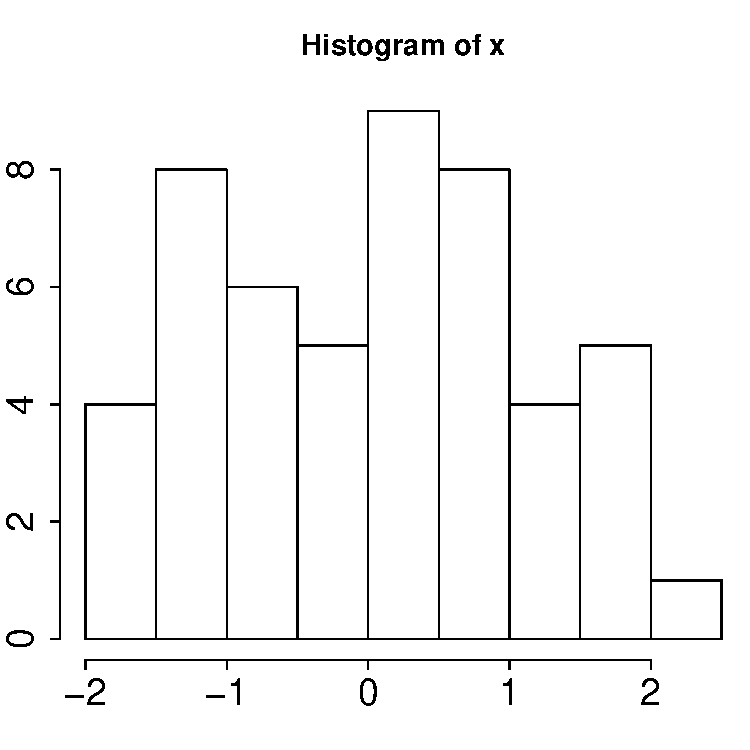
\includegraphics[width=\linewidth]{figure/graphics-pdf-hist1} 

}



\end{knitrout}

\caption{Histogram of 50 sampled values \label{mar:hist1}}
\end{marginfigure}


\vspace{0.25\textheight}


We can modify all the plots by providing certain arguments to the
plotting function. Now let's give a title to the plot using \emph{'main'}
argument. We can also change the color of the bars using \emph{'col'}
argument. You can simply provide the name of the color. Below, we
are using '\emph{red}' for the color. See Figure \ref{mar:hist_title}
for the result this chunk.

\begin{knitrout}
\definecolor{shadecolor}{rgb}{0.969, 0.969, 0.969}\color{fgcolor}\begin{kframe}
\begin{alltt}
\hlkwd{hist}\hlstd{(x,} \hlkwc{main} \hlstd{=} \hlstr{"Hello histogram!!!"}\hlstd{,} \hlkwc{col} \hlstd{=} \hlstr{"red"}\hlstd{)}
\end{alltt}
\end{kframe}
\end{knitrout}



\begin{marginfigure}
\begin{knitrout}
\definecolor{shadecolor}{rgb}{0.969, 0.969, 0.969}\color{fgcolor}

{\centering 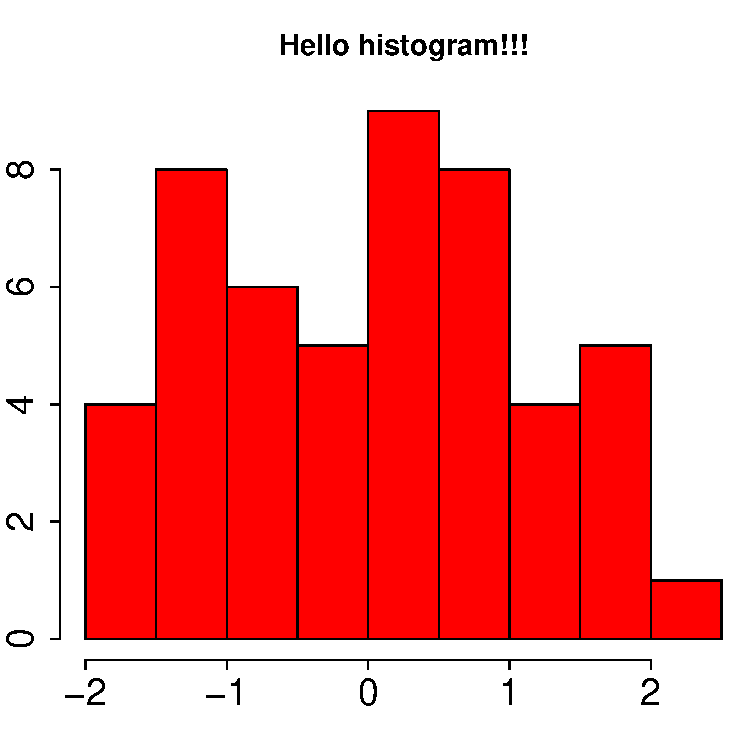
\includegraphics[width=\linewidth]{figure/graphics-pdf-hist2} 

}



\end{knitrout}



\caption{Histogram with a title\label{mar:hist_title}}
\end{marginfigure}


Next, we will plot a scatter plot. Scatter plots are one os the most
common plots you will encounter in data analysis. We will sample another
set of 50 values and plotted those against the ones we sampled earlier.
Scatterplot shows values of two variables for a set of data points.
It is useful to visualize relationships between two variables. It
is frequently used in connection with correlation and linear regression.
There are other variants of scatter plots which show density of the
points with different colors. We will show examples of those that
in following chapters. The scatter plot from our sampling experiment
is shown in Figure \ref{fig:scatter-plot-of}. Notice that, in addition
to main we used ``xlab'' and ``ylab'' arguments to give labels
to the plot. You can customize the plots even more than this. See
?plot and ?par for more arguments that can help you customize the
plots.

\begin{figure}
\begin{knitrout}
\definecolor{shadecolor}{rgb}{0.969, 0.969, 0.969}\color{fgcolor}\begin{kframe}
\begin{alltt}
\hlcom{# randomly sample 50 points from normal distribution }
\hlstd{y}\hlkwb{<-}\hlkwd{rnorm}\hlstd{(}\hlnum{50}\hlstd{)}
\hlcom{#plot a scatter plot }
\hlcom{# control x-axis and y-axis labels}
\hlkwd{plot}\hlstd{(x,y,}\hlkwc{main}\hlstd{=}\hlstr{"scatterplot of random samples"}\hlstd{,}
        \hlkwc{ylab}\hlstd{=}\hlstr{"y values"}\hlstd{,}\hlkwc{xlab}\hlstd{=}\hlstr{"x values"}\hlstd{)}
\end{alltt}
\end{kframe}

{\centering 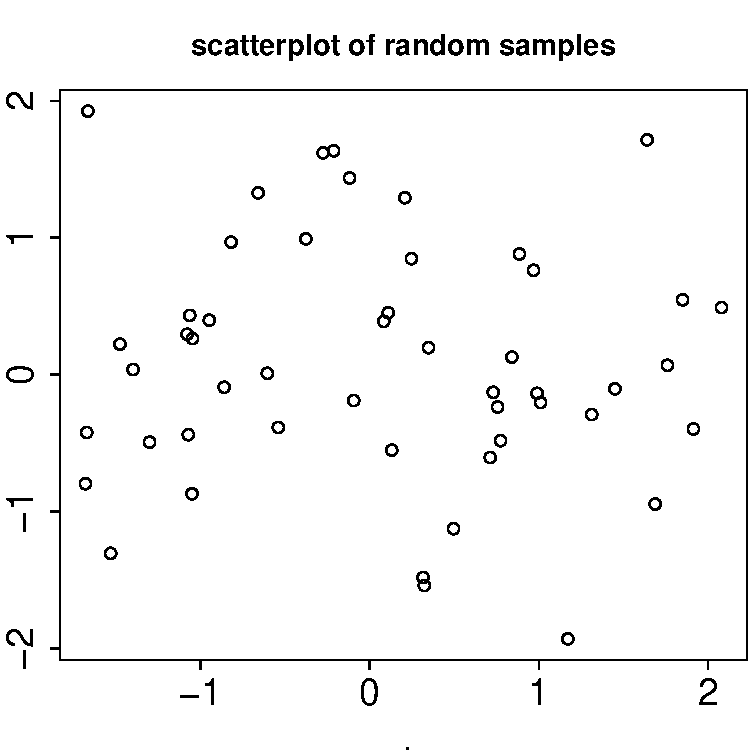
\includegraphics[width=2in,height=2in]{figure/graphics-scatter} 

}



\end{knitrout}


\caption{scatter plot of two random variables\label{fig:scatter-plot-of}}
\end{figure}


we can also plot boxplots for vectors \emph{x} and \emph{y.} Boxplots
depict groups of numerical data through their quartiles. The edges
of the box denote 1st and 3rd quartile, and the line that crosses
the box is the median. Whiskers usually are defined using interquantile
range,$lowerWhisker=Q1-1.5*IQR$ and $upperWhisker=Q1+1.5*IQR$. In
addition outliers can be depicted as dots. In this case, outliers
are the values that remain outside the whiskers.

\begin{figure}
\begin{knitrout}
\definecolor{shadecolor}{rgb}{0.969, 0.969, 0.969}\color{fgcolor}\begin{kframe}
\begin{alltt}
\hlkwd{boxplot}\hlstd{(x,y,}\hlkwc{main}\hlstd{=}\hlstr{"boxplots of random samples"}\hlstd{)}
\end{alltt}
\end{kframe}

{\centering 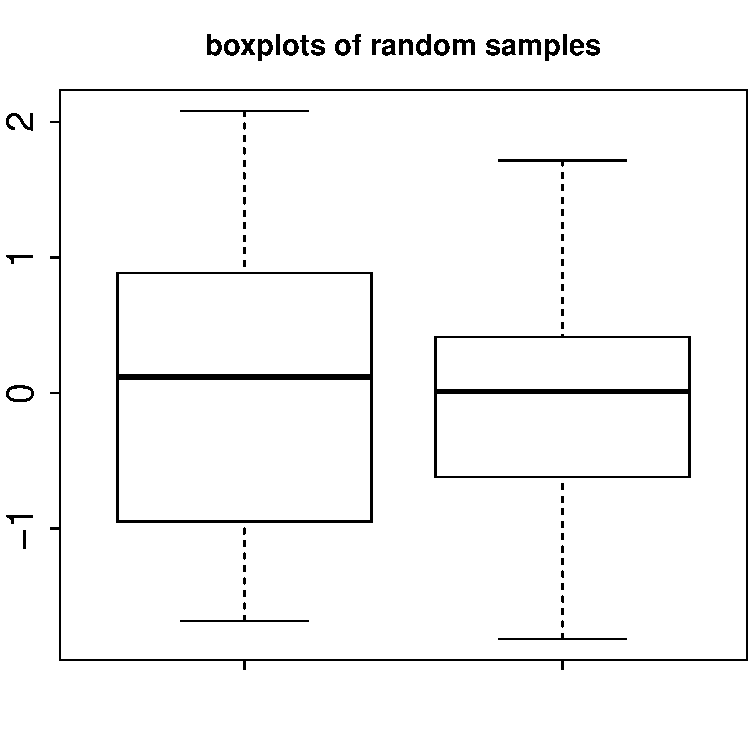
\includegraphics[width=2in]{figure/graphics-boxplot} 

}



\end{knitrout}


\caption{Boxplots for x and y vectors}
\end{figure}


Next up is bar plot which you can plot by barplot() function. We are
going to plot four imaginary percentage values and color them with
two colors, and this time we will also show how to draw a legend on
the plot using legend() function.

\begin{figure}
\begin{knitrout}
\definecolor{shadecolor}{rgb}{0.969, 0.969, 0.969}\color{fgcolor}\begin{kframe}
\begin{alltt}
\hlstd{perc}\hlkwb{=}\hlkwd{c}\hlstd{(}\hlnum{50}\hlstd{,}\hlnum{70}\hlstd{,}\hlnum{35}\hlstd{,}\hlnum{25}\hlstd{)}
\hlkwd{barplot}\hlstd{(}\hlkwc{height}\hlstd{=perc,}\hlkwc{names.arg}\hlstd{=}\hlkwd{c}\hlstd{(}\hlstr{"CpGi"}\hlstd{,}\hlstr{"exon"}\hlstd{,}\hlstr{"CpGi"}\hlstd{,}\hlstr{"exon"}\hlstd{),}
        \hlkwc{ylab}\hlstd{=}\hlstr{"percentages"}\hlstd{,}\hlkwc{main}\hlstd{=}\hlstr{"imagine %s"}\hlstd{,}
        \hlkwc{col}\hlstd{=}\hlkwd{c}\hlstd{(}\hlstr{"red"}\hlstd{,}\hlstr{"red"}\hlstd{,}\hlstr{"blue"}\hlstd{,}\hlstr{"blue"}\hlstd{))}
\hlkwd{legend}\hlstd{(}\hlstr{"topright"}\hlstd{,}\hlkwc{legend}\hlstd{=}\hlkwd{c}\hlstd{(}\hlstr{"test"}\hlstd{,}\hlstr{"control"}\hlstd{),}\hlkwc{fill}\hlstd{=}\hlkwd{c}\hlstd{(}\hlstr{"red"}\hlstd{,}\hlstr{"blue"}\hlstd{))}
\end{alltt}
\end{kframe}

{\centering 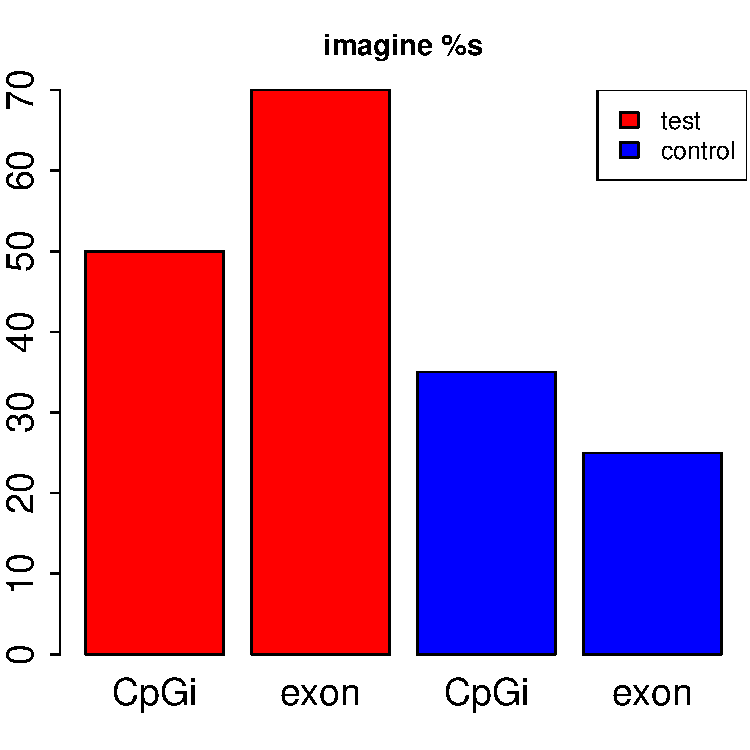
\includegraphics[width=2in]{figure/graphics-barplot} 

}



\end{knitrout}


\caption{Bar plot and legend example}
\end{figure}



\subsection{Saving Plots}

If you want to save your plots to an image file there are couple of
ways of doing that. Normally, you will have to do the following:

\begin{enumerate}
   \item Open a graphics device 
   \item Create the plot 
   \item Close the graphics device 
\end{enumerate}

\begin{knitrout}
\definecolor{shadecolor}{rgb}{0.969, 0.969, 0.969}\color{fgcolor}\begin{kframe}
\begin{alltt}
\hlkwd{pdf}\hlstd{(}\hlstr{"mygraphs/myplot.pdf"}\hlstd{,} \hlkwc{width} \hlstd{=} \hlnum{5}\hlstd{,} \hlkwc{height} \hlstd{=} \hlnum{5}\hlstd{)}
\hlkwd{plot}\hlstd{(x, y)}
\hlkwd{dev.off}\hlstd{()}
\end{alltt}
\end{kframe}
\end{knitrout}


Alternatively, you can first create the plot then copy the plot to
a graphical device.

\begin{knitrout}
\definecolor{shadecolor}{rgb}{0.969, 0.969, 0.969}\color{fgcolor}\begin{kframe}
\begin{alltt}
\hlkwd{plot}\hlstd{(x, y)}
\hlkwd{dev.copy}\hlstd{(pdf,} \hlstr{"mygraphs/myplot.pdf"}\hlstd{,} \hlkwc{width} \hlstd{=} \hlnum{7}\hlstd{,} \hlkwc{height} \hlstd{=} \hlnum{5}\hlstd{)}
\hlkwd{dev.off}\hlstd{()}
\end{alltt}
\end{kframe}
\end{knitrout}



\section{User defined functions}

Functions are useful for transforming larger chunks of code to re-usable
pieces of code. Generally, if you need to execute certain tasks with
variable parameters then it is time you write a function. A function
in R takes different arguments and returns a definite output, much
like mathematical functions. Here is a simple function takes two arguments,
x and y, and returns the sum of their squares.

\begin{knitrout}
\definecolor{shadecolor}{rgb}{0.969, 0.969, 0.969}\color{fgcolor}\begin{kframe}
\begin{alltt}
\hlstd{sqSum} \hlkwb{<-} \hlkwa{function}\hlstd{(}\hlkwc{x}\hlstd{,} \hlkwc{y}\hlstd{) \{}
    \hlstd{result} \hlkwb{<-} \hlstd{x}\hlopt{^}\hlnum{2} \hlopt{+} \hlstd{y}\hlopt{^}\hlnum{2}
    \hlkwd{return}\hlstd{(result)}
\hlstd{\}}
\hlcom{# now try the function out}
\hlkwd{sqSum}\hlstd{(}\hlnum{2}\hlstd{,} \hlnum{3}\hlstd{)}
\end{alltt}
\begin{verbatim}
## [1] 13
\end{verbatim}
\end{kframe}
\end{knitrout}


Functions can also output plots and/or messages to the terminal. Here
is a function that prints a message to the terminal:

\begin{knitrout}
\definecolor{shadecolor}{rgb}{0.969, 0.969, 0.969}\color{fgcolor}\begin{kframe}
\begin{alltt}
\hlstd{sqSumPrint} \hlkwb{<-} \hlkwa{function}\hlstd{(}\hlkwc{x}\hlstd{,} \hlkwc{y}\hlstd{) \{}
    \hlstd{result} \hlkwb{<-} \hlstd{x}\hlopt{^}\hlnum{2} \hlopt{+} \hlstd{y}\hlopt{^}\hlnum{2}
    \hlkwd{cat}\hlstd{(}\hlstr{"here is the result:"}\hlstd{, result,} \hlstr{"\textbackslash{}n"}\hlstd{)}
\hlstd{\}}
\hlcom{# now try the function out}
\hlkwd{sqSumPrint}\hlstd{(}\hlnum{2}\hlstd{,} \hlnum{3}\hlstd{)}
\end{alltt}
\begin{verbatim}
## here is the result: 13
\end{verbatim}
\end{kframe}
\end{knitrout}



\section{if-else control structures}

Sometimes we would want to execute a certain part of the code only
if certain condition is satisfied. This condition can be anything
from the type of an object (Ex: if object is a matrix execute certain
code), or it can be more compicated such as if object value is between
certain thresholds. Let us see how they can be used%
\footnote{see ?Control for more%
}. They can be used anywhere in your code, now we will use it in a
function.

\begin{knitrout}
\definecolor{shadecolor}{rgb}{0.969, 0.969, 0.969}\color{fgcolor}\begin{kframe}
\begin{alltt}
\hlcom{# function takes input one row of CpGi data frame}
\hlstd{largeCpGi} \hlkwb{<-} \hlkwa{function}\hlstd{(}\hlkwc{bedRow}\hlstd{) \{}
    \hlstd{cpglen} \hlkwb{<-} \hlstd{bedRow[}\hlnum{3}\hlstd{]} \hlopt{-} \hlstd{bedRow[}\hlnum{2}\hlstd{]} \hlopt{+} \hlnum{1}
    \hlkwa{if} \hlstd{(cpglen} \hlopt{>} \hlnum{1500}\hlstd{) \{}
        \hlkwd{cat}\hlstd{(}\hlstr{"this is large\textbackslash{}n"}\hlstd{)}
    \hlstd{\}} \hlkwa{else if} \hlstd{(cpglen} \hlopt{<=} \hlnum{1500} \hlopt{&} \hlstd{cpglen} \hlopt{>} \hlnum{700}\hlstd{) \{}
        \hlkwd{cat}\hlstd{(}\hlstr{"this is normal\textbackslash{}n"}\hlstd{)}
    \hlstd{\}} \hlkwa{else} \hlstd{\{}
        \hlkwd{cat}\hlstd{(}\hlstr{"this is short\textbackslash{}n"}\hlstd{)}
    \hlstd{\}}
\hlstd{\}}
\hlkwd{largeCpGi}\hlstd{(cpgi.df[}\hlnum{10}\hlstd{, ])}
\hlkwd{largeCpGi}\hlstd{(cpgi.df[}\hlnum{100}\hlstd{, ])}
\hlkwd{largeCpGi}\hlstd{(cpgi.df[}\hlnum{1000}\hlstd{, ])}
\end{alltt}
\end{kframe}
\end{knitrout}



\section{Loops and looping structures in R}

When you need to repeat a certain task or a execute a function multiple
times, you can do that with the help of loops. A loop will execute
the task until a certain condition is reached. The loop below is called
a ``for-loop'' and it executes the task sequentially 10 times.

\begin{knitrout}
\definecolor{shadecolor}{rgb}{0.969, 0.969, 0.969}\color{fgcolor}\begin{kframe}
\begin{alltt}
\hlkwa{for} \hlstd{(i} \hlkwa{in} \hlnum{1}\hlopt{:}\hlnum{10}\hlstd{) \{}
    \hlcom{# number of repetitions}
    \hlkwd{cat}\hlstd{(}\hlstr{"This is iteration"}\hlstd{)}  \hlcom{# the task to be repeated}
    \hlkwd{print}\hlstd{(i)}
\hlstd{\}}
\end{alltt}
\begin{verbatim}
## This is iteration[1] 1
## This is iteration[1] 2
## This is iteration[1] 3
## This is iteration[1] 4
## This is iteration[1] 5
## This is iteration[1] 6
## This is iteration[1] 7
## This is iteration[1] 8
## This is iteration[1] 9
## This is iteration[1] 10
\end{verbatim}
\end{kframe}
\end{knitrout}


The task above is a bit pointless, normally in a loop, you would want
to do something meaningful. Let us calculate the length of the CpG
islands we read in earlier. Although this is not the most efficient
way of doing that particular task, it serves as a good example for
looping. The code below will be execute hundred times, and it will
calculate the length of the CpG islands for the first 100 islands
in the data frame (by subtracting the end coordinate from the start
coordinate) %
\footnote{\uline{TIP:} If you are going to run a loop that has a lot of repetitions,
it is smart to try the loop with few repetitions first and check the
results. This will help you make sure the code in the loop works before
executing it for thousands of times.%
}.

\begin{knitrout}
\definecolor{shadecolor}{rgb}{0.969, 0.969, 0.969}\color{fgcolor}\begin{kframe}
\begin{alltt}
\hlcom{# this is where we will keep the lenghts for now it}
\hlcom{# is an empty vector}
\hlstd{result} \hlkwb{<-} \hlkwd{c}\hlstd{()}
\hlcom{# start the loop}
\hlkwa{for} \hlstd{(i} \hlkwa{in} \hlnum{1}\hlopt{:}\hlnum{100}\hlstd{) \{}
    \hlcom{# calculate the length}
    \hlstd{len} \hlkwb{<-} \hlstd{cpgi.df[i,} \hlnum{3}\hlstd{]} \hlopt{-} \hlstd{cpgi.df[i,} \hlnum{2}\hlstd{]} \hlopt{+} \hlnum{1}
    \hlcom{# append the length to the result}
    \hlstd{result} \hlkwb{<-} \hlkwd{c}\hlstd{(result, len)}
\hlstd{\}}
\hlcom{# check the results}
\hlkwd{head}\hlstd{(result)}
\end{alltt}
\begin{verbatim}
## [1]  277  360  383 1325 3498 1602
\end{verbatim}
\end{kframe}
\end{knitrout}



\subsection{apply family functions instead of loops}

R has other ways of repeating tasks that tend to be more efficient
than using loops. They are known as the \emph{``apply''} family
of functions, which include \emph{apply,lapply, mapply and tapply}
(and some other variants)\emph{.} All of these functions apply a given
function to a set of instances and returns the result of those functions
for each instance. The differences between them is that they take
different type of inputs. For example apply works on data frames or
matrices and applies the function on each row or column of the data
structure. lapply works on lists or vectors and applies a function
which takes the list element as an argument. Next we will demonstrate
how to use apply() on a matrix. The example applies the sum function
on the rows of a matrix, it basically sums up the values on each row
of the matrix, which is conceptualized in Figure \ref{mar:apply-on-a-matrix}

\begin{marginfigure}
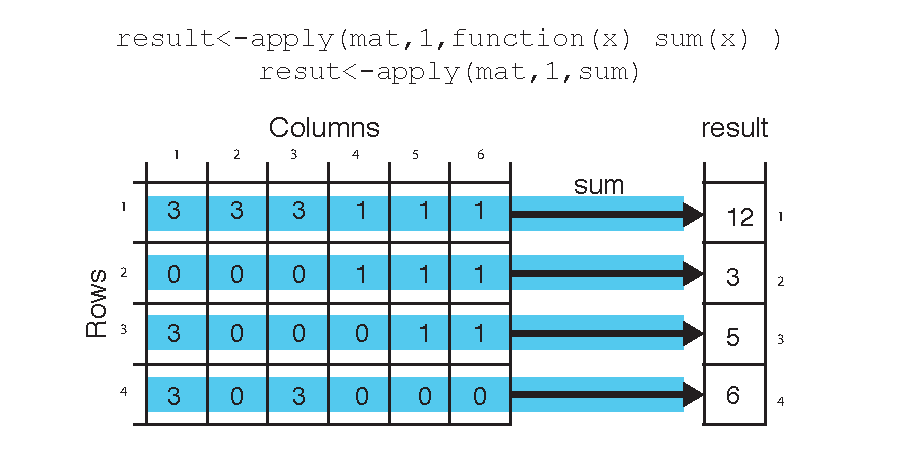
\includegraphics[clip,scale=0.5]{1_Users_altuna_Dropbox_PAPERS_R-devel_compgenr_chapters_nonR_figures_apply.pdf}\caption{apply on rows\label{mar:apply-on-a-matrix}}


\end{marginfigure}


\begin{knitrout}
\definecolor{shadecolor}{rgb}{0.969, 0.969, 0.969}\color{fgcolor}\begin{kframe}
\begin{alltt}
\hlstd{mat} \hlkwb{<-} \hlkwd{cbind}\hlstd{(}\hlkwd{c}\hlstd{(}\hlnum{3}\hlstd{,} \hlnum{0}\hlstd{,} \hlnum{3}\hlstd{,} \hlnum{3}\hlstd{),} \hlkwd{c}\hlstd{(}\hlnum{3}\hlstd{,} \hlnum{0}\hlstd{,} \hlnum{0}\hlstd{,} \hlnum{0}\hlstd{),} \hlkwd{c}\hlstd{(}\hlnum{3}\hlstd{,} \hlnum{0}\hlstd{,}
    \hlnum{0}\hlstd{,} \hlnum{3}\hlstd{),} \hlkwd{c}\hlstd{(}\hlnum{1}\hlstd{,} \hlnum{1}\hlstd{,} \hlnum{0}\hlstd{,} \hlnum{0}\hlstd{),} \hlkwd{c}\hlstd{(}\hlnum{1}\hlstd{,} \hlnum{1}\hlstd{,} \hlnum{1}\hlstd{,} \hlnum{0}\hlstd{),} \hlkwd{c}\hlstd{(}\hlnum{1}\hlstd{,} \hlnum{1}\hlstd{,} \hlnum{1}\hlstd{,}
    \hlnum{0}\hlstd{))}
\hlstd{result} \hlkwb{<-} \hlkwd{apply}\hlstd{(mat,} \hlnum{1}\hlstd{, sum)}
\hlstd{result}
\end{alltt}
\begin{verbatim}
## [1] 12  3  5  6
\end{verbatim}
\begin{alltt}
\hlcom{# OR you can define the function as an argument to}
\hlcom{# apply()}
\hlstd{result} \hlkwb{<-} \hlkwd{apply}\hlstd{(mat,} \hlnum{1}\hlstd{,} \hlkwa{function}\hlstd{(}\hlkwc{x}\hlstd{)} \hlkwd{sum}\hlstd{(x))}
\hlstd{result}
\end{alltt}
\begin{verbatim}
## [1] 12  3  5  6
\end{verbatim}
\end{kframe}
\end{knitrout}


Notice that we used a second argument which equals to 1, that indicates
that rows of the matrix/ data frame will be the input for the function.
If we change the second argument to 2, this will indicate that columns
should be the input for the function that will be applied. See Figure
\ref{mar:apply-on-columns} for the visualization of apply() on columns.

\begin{knitrout}
\definecolor{shadecolor}{rgb}{0.969, 0.969, 0.969}\color{fgcolor}\begin{kframe}
\begin{alltt}
\hlstd{result} \hlkwb{<-} \hlkwd{apply}\hlstd{(mat,} \hlnum{2}\hlstd{, sum)}
\hlstd{result}
\end{alltt}
\begin{verbatim}
## [1] 9 3 6 2 3 3
\end{verbatim}
\end{kframe}
\end{knitrout}


\begin{marginfigure}
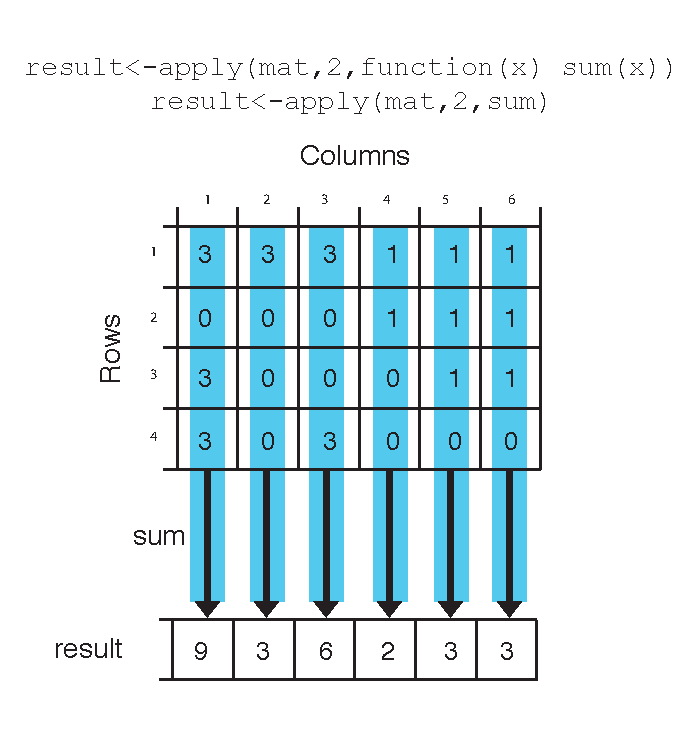
\includegraphics[clip,scale=0.5]{2_Users_altuna_Dropbox_PAPERS_R-devel_compgenr_chapters_nonR_figures_apply2.pdf}

\caption{apply on columns\label{mar:apply-on-columns}}
\end{marginfigure}


next we will use lapply, which applies a function on a list or a vector.
The function that will be applied is a simple function that takes
the square of a given number.

\begin{knitrout}
\definecolor{shadecolor}{rgb}{0.969, 0.969, 0.969}\color{fgcolor}\begin{kframe}
\begin{alltt}
\hlstd{input} \hlkwb{<-} \hlkwd{c}\hlstd{(}\hlnum{1}\hlstd{,} \hlnum{2}\hlstd{,} \hlnum{3}\hlstd{)}
\hlkwd{lapply}\hlstd{(input,} \hlkwa{function}\hlstd{(}\hlkwc{x}\hlstd{) x}\hlopt{^}\hlnum{2}\hlstd{)}
\end{alltt}
\begin{verbatim}
## [[1]]
## [1] 1
## 
## [[2]]
## [1] 4
## 
## [[3]]
## [1] 9
\end{verbatim}
\end{kframe}
\end{knitrout}


mapply is another member of apply family, it can apply a function
on an unlimited set of vectors/lists, it is like a version of lapply
that can handle multiple vectors as arguments. In this case, the argument
to the mapply() is the function to be applied and the sets of parameters
to be supplied as arguments of the function. This conceptualized Figure
\ref{mar:mapply-takes-in}, the function to be applied is a function
that takes to arguments and sums them up. The arguments to be summed
up are in the format of vectors, Xs and Ys. mapply() applies the summation
function to each pair in Xs and Ys vector. Notice that the order of
the input function and extra arguments are different for mapply.

\begin{knitrout}
\definecolor{shadecolor}{rgb}{0.969, 0.969, 0.969}\color{fgcolor}\begin{kframe}
\begin{alltt}
\hlstd{Xs} \hlkwb{<-} \hlnum{0}\hlopt{:}\hlnum{5}
\hlstd{Ys} \hlkwb{<-} \hlkwd{c}\hlstd{(}\hlnum{2}\hlstd{,} \hlnum{2}\hlstd{,} \hlnum{2}\hlstd{,} \hlnum{3}\hlstd{,} \hlnum{3}\hlstd{,} \hlnum{3}\hlstd{)}
\hlstd{result} \hlkwb{<-} \hlkwd{mapply}\hlstd{(}\hlkwa{function}\hlstd{(}\hlkwc{x}\hlstd{,} \hlkwc{y}\hlstd{)} \hlkwd{sum}\hlstd{(x, y), Xs, Ys)}
\hlstd{result}
\end{alltt}
\begin{verbatim}
## [1] 2 3 4 6 7 8
\end{verbatim}
\end{kframe}
\end{knitrout}


\begin{marginfigure}
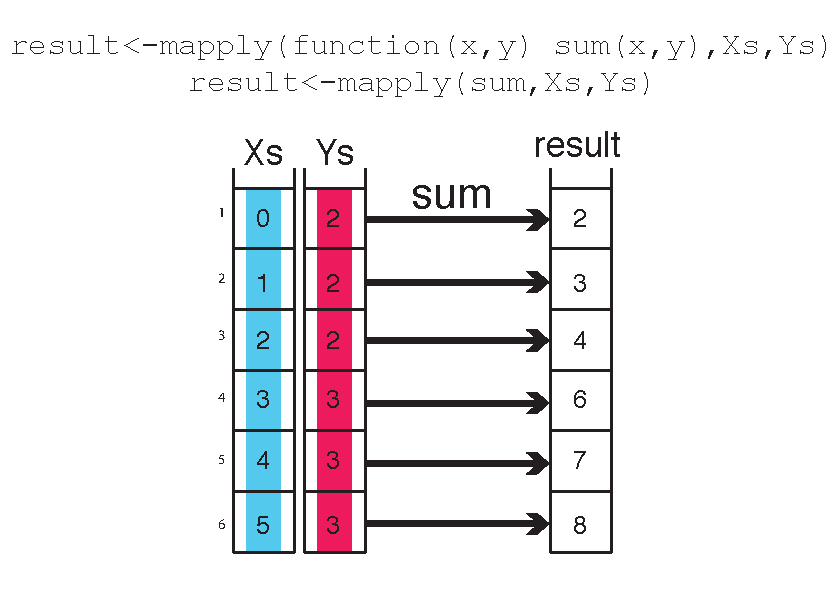
\includegraphics[clip,scale=0.5]{3_Users_altuna_Dropbox_PAPERS_R-devel_compgenr_chapters_nonR_figures_mapply.pdf}

\caption{mapply takes in multiple/vectors and lists\label{mar:mapply-takes-in}}
\end{marginfigure}



\subsection{apply family functions on multiple cores}

If you have large data sets apply-family functions can be slow (although
probably still better than for loops). If that is the case, you can
easily use the parallel versions of those functions from parallel
package. These functions essentially divide your tasks to smaller
chunks run them on separate CPUs and merge the results from those
parallel operations. This concept is visualized at Figure \ref{mar:mcmapply-on-3},
mcapply runs the summation function on three different processors.
Each processor executes the summation function on a part of the data
set, and the results are merged and returned as a single vector that
has the same order as the input parameters Xs and Ys.

\begin{marginfigure}
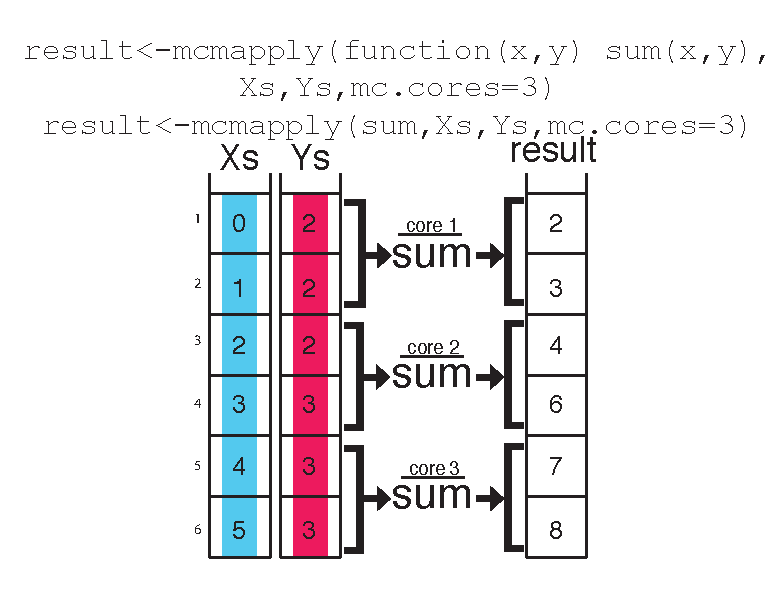
\includegraphics[scale=0.5]{4_Users_altuna_Dropbox_PAPERS_R-devel_compgenr_chapters_nonR_figures_mcmapply.pdf}

\caption{mcmapply on 3 cores\label{mar:mcmapply-on-3}}
\end{marginfigure}



\subsection{Vectorized functions in R}

The above examples have been put forward to illustrate functions and
loops in R because functions using sum() are not complicated and easy
to understand. You will probably need to use loops and looping structures
with more complicated functions. In reality, most of the operations
we used do not need the use of loops or looping structures because
there are already vectorized functions that can achieve the same outcomes,
meaning if the input arguments are R vectors the output will be a
vector as well, so no need for loops or vectorization.

For example, instead of using mapply() and sum() functions we can
just use + operator and sum up Xs and Ys. 

\begin{knitrout}
\definecolor{shadecolor}{rgb}{0.969, 0.969, 0.969}\color{fgcolor}\begin{kframe}
\begin{alltt}
\hlstd{result} \hlkwb{<-} \hlstd{Xs} \hlopt{+} \hlstd{Ys}
\hlstd{result}
\end{alltt}
\begin{verbatim}
## [1] 2 3 4 6 7 8
\end{verbatim}
\end{kframe}
\end{knitrout}


In order to get the column or row sums, we can use the vectorized
functions colSums() and rowSums()

\begin{knitrout}
\definecolor{shadecolor}{rgb}{0.969, 0.969, 0.969}\color{fgcolor}\begin{kframe}
\begin{alltt}
\hlkwd{colSums}\hlstd{(mat)}
\end{alltt}
\begin{verbatim}
## [1] 9 3 6 2 3 3
\end{verbatim}
\begin{alltt}
\hlkwd{rowSums}\hlstd{(mat)}
\end{alltt}
\begin{verbatim}
## [1] 12  3  5  6
\end{verbatim}
\end{kframe}
\end{knitrout}


However, remember that not every function is vectorized in R, use
the ones that are. But sooner or later, apply family functions will
come in handy.


\section{Session Info}

\begin{knitrout}
\definecolor{shadecolor}{rgb}{0.969, 0.969, 0.969}\color{fgcolor}\begin{kframe}
\begin{alltt}
\hlkwd{sessionInfo}\hlstd{()}
\end{alltt}
\begin{verbatim}
## R version 3.0.2 (2013-09-25)
## Platform: x86_64-apple-darwin10.8.0 (64-bit)
## 
## locale:
## [1] C
## 
## attached base packages:
## [1] parallel  methods   stats     graphics 
## [5] grDevices utils     datasets  base     
## 
## other attached packages:
## [1] codetools_0.2-8       Rsamtools_1.13.49    
## [3] GenomicRanges_1.13.51 Biostrings_2.29.19   
## [5] XVector_0.1.4         IRanges_1.19.38      
## [7] BiocGenerics_0.7.5    knitr_1.5            
## 
## loaded via a namespace (and not attached):
## [1] bitops_1.0-6   digest_0.6.3   evaluate_0.5  
## [4] formatR_0.9    highr_0.2.1    stats4_3.0.2  
## [7] stringr_0.6.2  tools_3.0.2    zlibbioc_1.7.0
\end{verbatim}
\end{kframe}
\end{knitrout}



\section{Acknowledgements}

Chapter is initiated by Altuna Akalin.
\end{document}
